% !TeX root = ../main.tex

\chapter{Introduction}

Rapid advances in machine learning have enabled computer models to solve tasks that previously necessitated extensive human labor. Most of such successes rely on supervised learning, a learning paradigm in which computer models are trained on labeled data. These labeled data guide these models to learn efficiently. However, labeling data is challenging and laborious. For example, to train a model to predict the solubility of a chemical compound, experts need some domain knowledge about chemistry to label data on molecular attributes before training. The cost of labeling data makes supervised learning less attractive and robust.

Recently, learning from unlabeled data has become popular in machine learning. One of such learning concepts is called self-supervised learning, which trains models by leveraging information from data themselves without guidance from labels or other external information. Models trained by self-supervised learning are often used to produce a data representation, i.e., features, for various downstream tasks such as prediction and classification. 

Generally, self-supervised learning methods can be grouped into four approaches: contrastive learning, clustering learning, distillation learning, and redundancy reduction. In the fields of computer vision (CV) \cite{sslcv} and natural language processing (NLP), researchers have developed many self-supervised methods. These methods have produced models that outperform other supervised learning methods in many benchmark tasks. 

However, despite its widespread use in computer vision and NLP, self-supervised learning remains a challenge in graph representation learning. One early attempt is the GraphCL \cite{GraphCL} introduced by You et al.  The GraphCL method trains graph neural networks (GNNs) under a contrastive learning framework. It has achieved remarkable results in several graph classification benchmarks. 

In this thesis, we use three self-supervised learning approaches to train models on graph data: contrastive learning, distillation learning, and redundancy reduction. We will conduct simulation experiments by training our models on four real-world datasets under various experimental settings: the use of different data augmentation methods, different numbers of layers, various batch sizes, and so on. Overall, there are 144 experimental settings. Figure \ref{fig:exp} shows the flow diagram of each experiment.

\begin{figure}[!htbp]
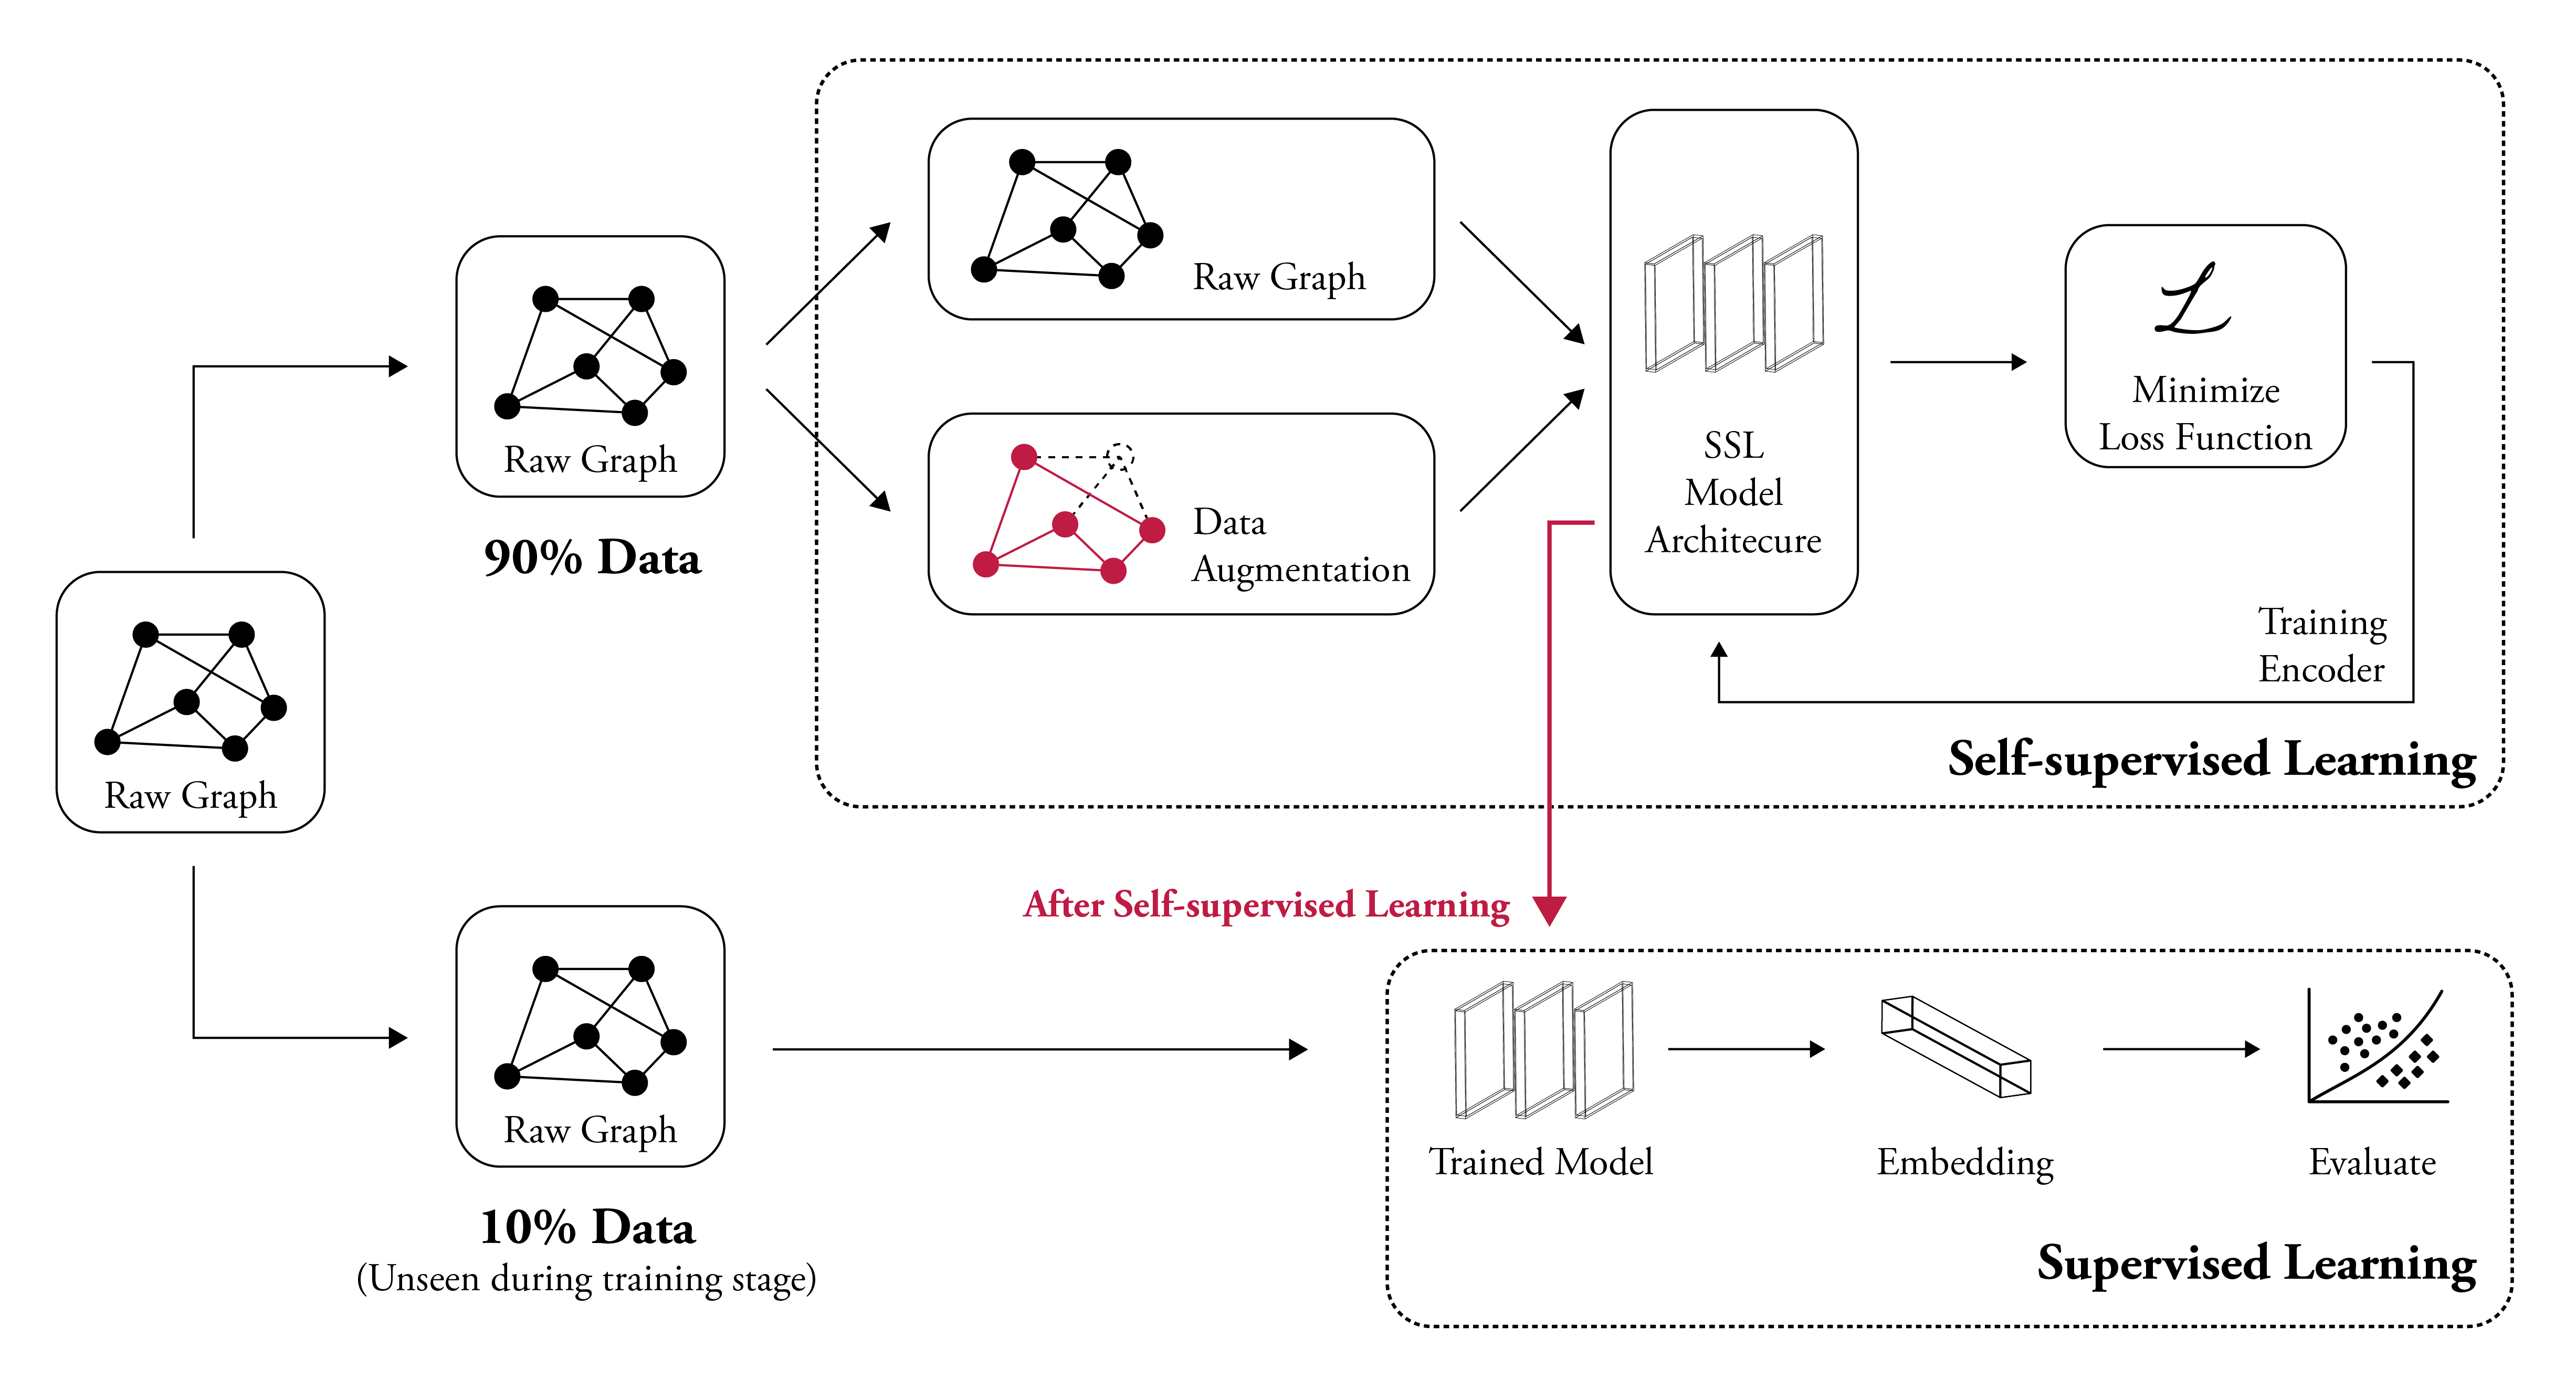
\includegraphics[width=\textwidth]{./figures/guide-02.png}
\caption[Flow diagram of experiments]{\textbf{Flow diagram of experiments.}  The experiment can be roughly separated into two parts: 90\% of the data are used to train an encoder via self-supervised learning, and the other 10\% are used to evaluate the performance of the model via supervised learning. }
\label{fig:exp}
\end{figure}

This thesis comprises five themed chapters. In the next chapter, we will review self-supervised learning and benchmark GNN models, which serve as encoders for extracting features from graph data. Then, we will describe three self-supervised learning methods in Chapter 3 that will be further used to train GNNs on unlabeled data. In Chapter 4, we will evaluate the performance of the three self-supervised learning methods by conducting simulation experiments, where several GNNs will be trained on real-world data under different experiment settings. Finally, we will briefly describe possible future research directions in the last chapter as a conclusion.




